\section{Benchmarks}

The following benchmarks were performed individually for each of the previously mentioned kernel modifications on an Arch Linux Virtual Machine. To empirically measure the throughput and turnaround time of various workloads, Prime95 was used to stress test the various kernel builds. In addition, a custom built C++ program was used to run a synthetic workload on 16 concurrent child processes, and calculated the average time required to finish each process.

The benchmarks used were as follows:
\begin{itemize}
	\item Prime 95 Benchmark, sampled when running 25 iterations of 2048K FFT on 1, 2 and 4 cores.
	\item SyntheticProcess, our custom C++ synthetic load program, running 16 child processes each running a synthetic load and then averaging the completion time of all children (with a 1 sec delay between iterations to ensure the children were dequeued completely).
	\item A composite test where Prime 95 and SyntheticProcess are run in parallel to evaluate CFS's ability to share between entirely separate pid parents.
\end{itemize}

\noindent The Kernels used in our benchmarks were as follows:
\begin{description}
	\item[STOCK] A stock build of Linux 4.2.6
	\item[Test1] A modified version of the stock Kernel, implementing the pick\_next\_task psudocode changes detailed above.
	\item[Test2] A stock build of Linux 4.2.6 with the following kernel parameters configured using \texttt{sysctl}:
	
		sched\_rt\_period\_us = 10,
		
		sched\_rt\_runtime\_us = 10,
		
		sched\_rr\_timeslice\_ms = 1,
		
		sched\_cfs\_bandwidth\_slice\_us = 1
	\item[Test3] A modified version of the stock Kernel, implementing the CFS Bandwidth and Quota changes detailed above. Specifically, RUNTIME\_INF was set to 10\% of the CFS bandwidth period (previously it was unrestricted), refill\_cfs\_bandwidth\_runtime() was short circuited to disable refilling alloted bandwidth, and the sched.h preprocessor constant MAX\_SHARES was changed from 2\^18 to 2\^9.
\end{description}

\textbf{Benchmark Results}

\begin{figure}[hb]
	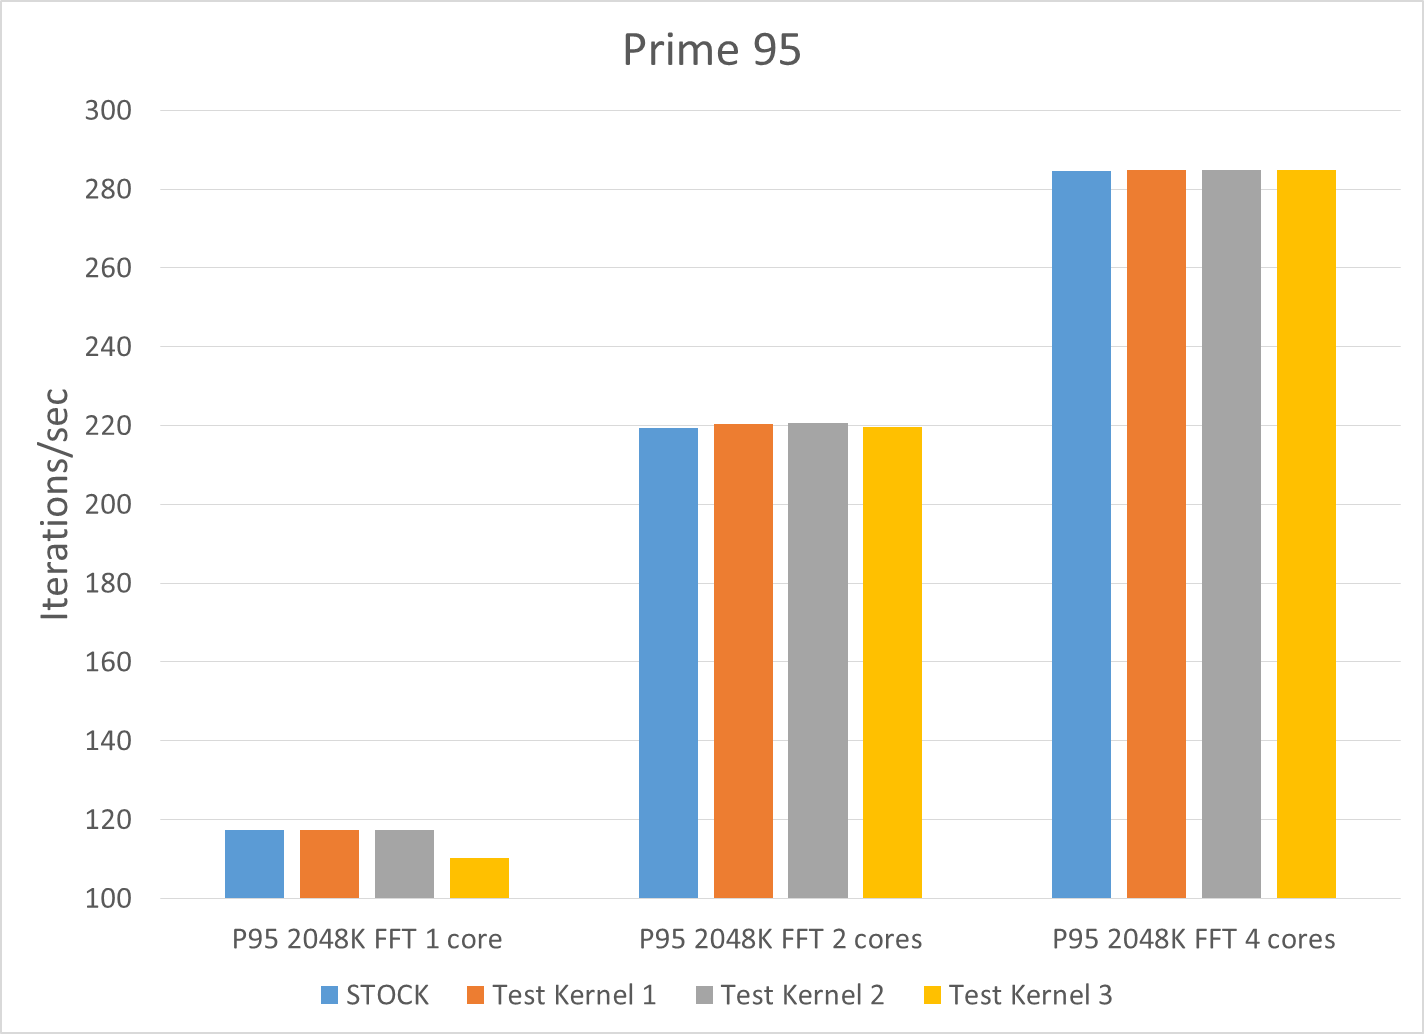
\includegraphics[width=1.0\columnwidth]{images/P95}
	\caption{Displaying the default values for the stock Arch Linux Kernel}
\end{figure}

\begin{figure}[hb]
	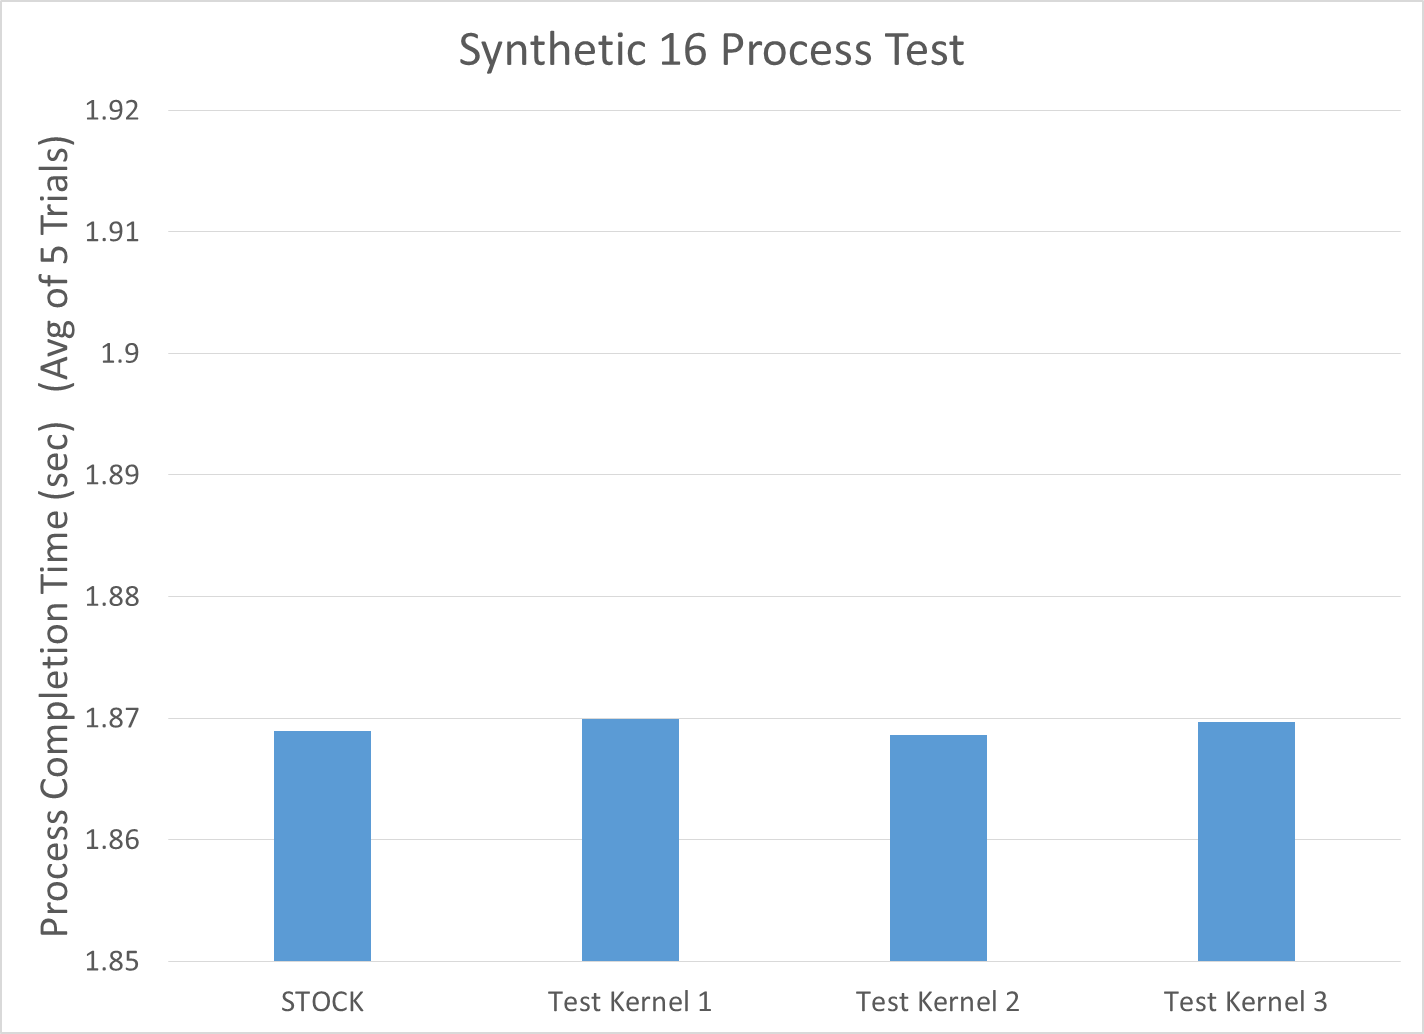
\includegraphics[width=1.0\columnwidth]{images/Synthetic}
	\caption{Displaying the default values for the stock Arch Linux Kernel}
\end{figure}

\begin{figure}[hb]
	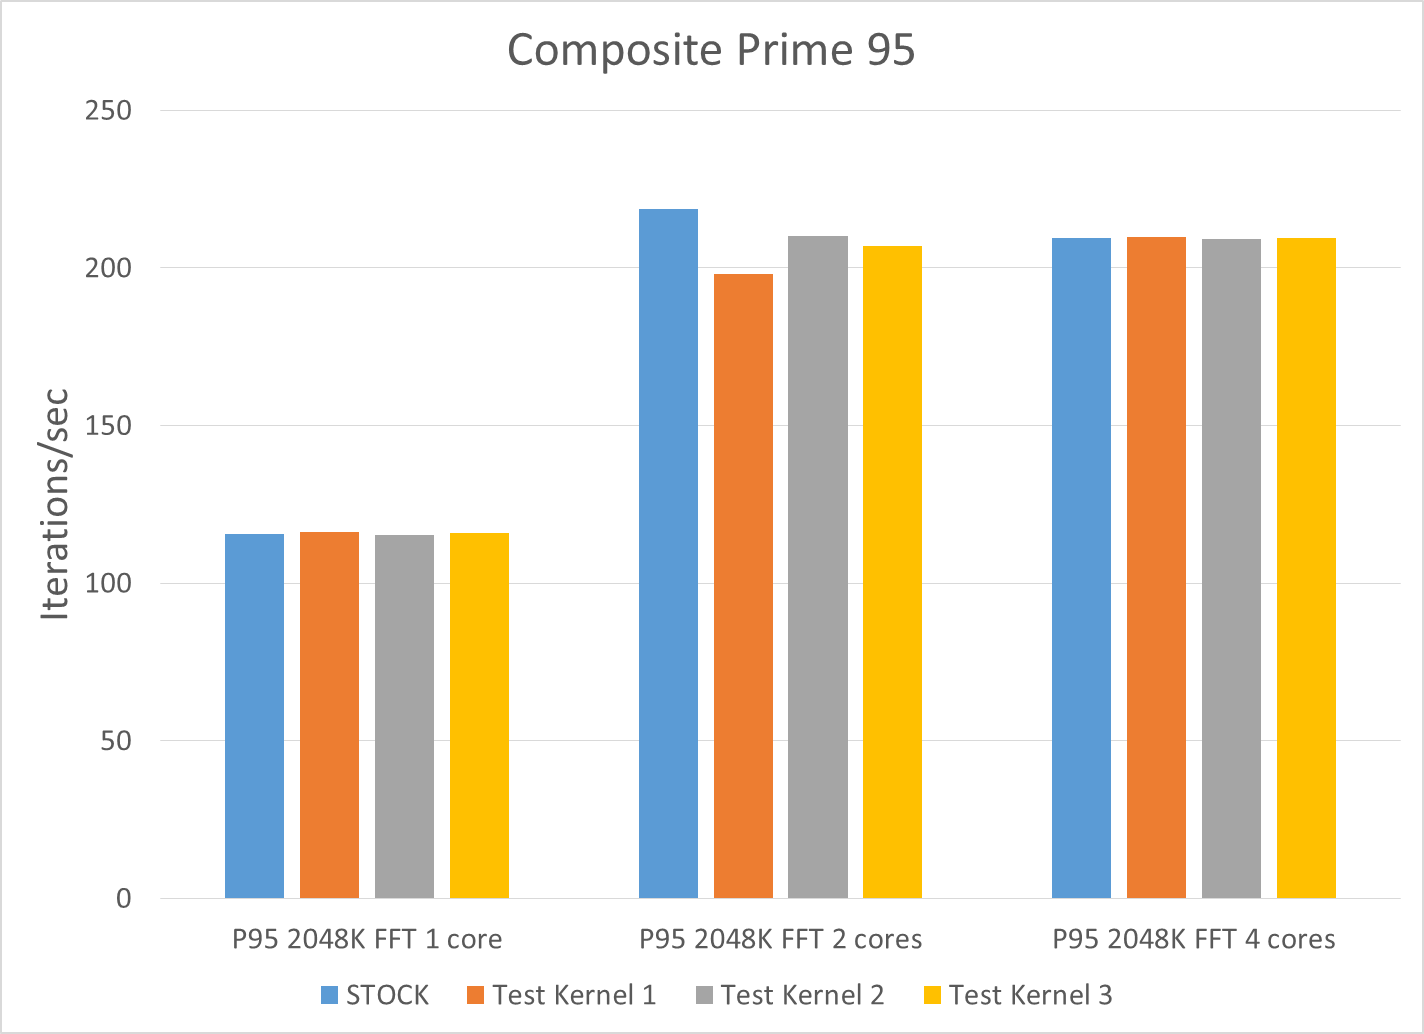
\includegraphics[width=1.0\columnwidth]{images/CompositeP95}
	\caption{Displaying the default values for the stock Arch Linux Kernel}
\end{figure}

\begin{figure}[hb]
	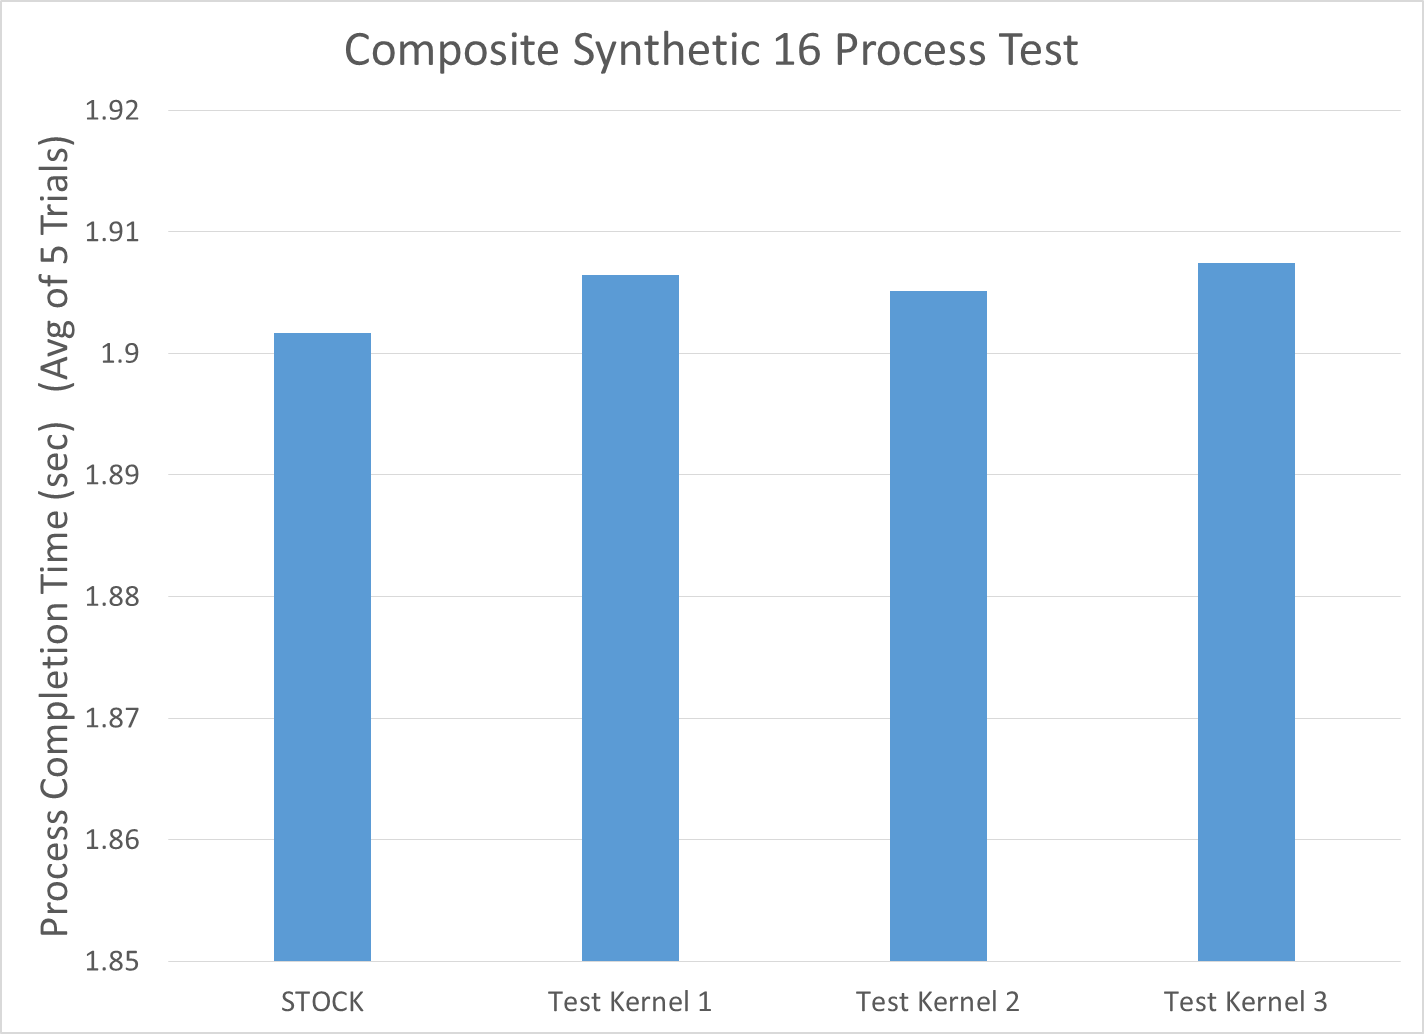
\includegraphics[width=1.0\columnwidth]{images/CompositeSynthetic}
	\caption{Displaying the default values for the stock Arch Linux Kernel}
\end{figure}